%/* vim: set ai tw=75: */%  -*- fill-column: 75 -*-
%% $Id$
\documentclass[a4paper,onecolumn,oneside,12pt]{mwart}
\usepackage[MeX]{polski}
\usepackage[utf8]{inputenc}
\usepackage{url}
\usepackage{listings}
\usepackage{graphicx}
\usepackage[lmargin=3.5cm,rmargin=2.5cm,tmargin=3cm,bmargin=2cm]{geometry}
\usepackage{verbatim}
\usepackage{color}
\usepackage{setspace}

\author{Michał Nazarewicz \and Maciej Andrzej Świętochowski}
\title{Wizualizacja 3D grafu}
\date{\today}

\definecolor{gray95}{gray}{0.95}

\lstset{breaklines=true,breakindent=0pt ,prebreak=\mbox{},
postbreak=\mbox{}, basicstyle={\ttfamily}, frame=lines,
basewidth={0.5em, 0.4em}, tabsize=4}

\begin{document}

\maketitle

\section{Szczegółowy opis zadania}

Zadanie polega na zaprojektowaniu i wykonaniu programu umożliwiającego
trójwymiarową wizualizację grafu. Program powinien mieć możliwość
wygenerowania grafu według zadanych parametrów oraz wczytywania grafu z
pliku o ustalonym formacie. Wizualizacja grafu powinna być ,,ładna'' --
czytelna, przejrzysta. Opracowanie mierzalnych kryteriów, które
wizualizacja musi spełniać również jest częścią zadania.

\section{Założenia projektu}

Program zostanie wykonany w języku C++ z~wykorzystaniem bibliotek: Qt
(interfejs graficzny), OpenGL (renderowanie sceny 3D) oraz GNU Scientific
Library (generowanie liczb pseudolosowych). Program będzie
przetwarzał grafy spójne, nieskierowane, bez wag krawędziowych lub
wierzchołkowych. Zadanie wizualizacji 3D polega na przypisaniu każdemu
wierzchołkowi uporządkowanej trójki współrzędnych oraz wyświetleniu rzutu
tej przestrzeni na obszar dwuwymiarowy według zadanych przez użytkownika
parametrów. W celu ułatwienia zmiany tych parametrów program będzie
wyposażony w graficzny interfejs użytkownika, a najprostsze parametry (wizualnie
odpowiadające za przesunięcie, skalowanie i obrót płaszczyzny, na którą
widok będzie rzutowany) będą ustalane przy pomocy urządzenia wskazującego
(,,myszy'' komputerowej). Poszukiwania wizualizacji grafu będą prowadzone
wg modelu fizycznego (por. \ref{model:physics}) oraz ewolucyjnego (por.
\ref{model:optimize}).

\subsection{Generowanie grafów}
Program będzie umożliwiał generowanie grafów Euklidesowych, w sposób
następujący:
\begin{itemize}
	\item wygenerowanie z zadanym rozkładem punktów $v$ w przestrzeni trójwymiarowej
    (sześcian o boku jednostkowym),
	\item dla każdego punktu $v$: wyszukanie zbioru $W_v$ punktów $w_i$
		sąsiednich względem $v$, tzn. takich, które należą do sferycznego
		sąsiedztwa o promieniu $r$ punktu $v$,
	\item dla każdego punktu $v$: losowe przypisanie każdej parze $(v,
		w_i)$ wartości $0$ lub $1$ tak, że prawdopodobieństwo wylosowania
		wartości $1$ maleje wraz z Euklidesową odległością pomiędzy
		punktami $v$ i $w_i$ w przestrzeni (rodzaj zależności będzie parametryzowalny)
	\item punkty $v$ stają się wierzchołkami grafu, a pary $(v, w_i)$,
		którym przypisano wartość $1$ stają się krawędziami grafu.
\end{itemize}

\subsection{Wizualizacja 3D}

Podstawowym problemem przy wizualizacji 3D grafu jest przypisanie jego
wierzchołkom współrzędnych przestrzeni trójwymiarowej. Najprostszą
przestrzenną reprezentacją wierzchołków są kule, a reprezentacją krawędzi
-- linie lub walce. Chcielibyśmy, aby wizualizacja grafu była ,,ładna'', to
znaczy spełniała pewne warunki, które są dla odbiorcy oczywiste,
intuicyjne. Poniżej zamieszczamy kilka takich oczywistych warunków,
utożsamiając pojęcie wierzchołka i krawędzi z reprezentacją graficzną
wierzchołka i reprezentacją graficzną krawędzi:
\begin{itemize}
	\item wierzchołki nie powinny na siebie zachodzić,
	\item krawędzie nie powinny się przecinać,
	\item krawędzie powinny być jak najkrótsze, przyjmując pewną minimalną
		ich długość,
	\item wierzchołki odległe w sensie najkrótszej ścieżki pomiędzy nimi
		powinny być odległe według miary Euklidesowej.
\end{itemize}
Powyższa lista nie jest zamknięta, opracowanie dokładnych kryteriów również
jest częścią zadania i będzie dokonane częściowo w formie eksperymentu.

Oczywistym jest, że wizualizacji grafu, które spełniają podane kryteria,
jest nieskończenie wiele. W związku z tym należy wybrać jedną z nich w
sposób automatyczny. Możliwe są dwa modele: fizyczny, oraz optymalizacyjny.

\subsubsection{Model fizyczny}
\label{model:physics}

W modelu fizycznym zakładamy, że wierzchołki wzajemnie na siebie
oddziałują, a rodzaj i siła tych oddziaływań jest uzależniona od relacji
pomiędzy nimi (sąsiedztwo). W tym modelu znalezienie wizualizacji polega na
znalezieniu położenia równowagi układu wierzchołków, tzn sytuacji, w której
wierzchołki przestają się poruszać, tj. gdy energia kinetyczna układu jest
bliska zeru.

Pewnym problemem związanym ze stosowaniem tego modelu jest fakt, iż nie są
brane pod uwagę krawędzie, a chcielibyśmy, by się one co najmniej nie
przecinały.

\subsubsection{Model optymalizacyjny}
\label{model:optimize}

Model optymalizacyjny zakłada, że umiemy skonstruować funkcję oceny, która
określa jak ,,ładna'' jest dowolna wizualizacja. Znalezienie odpowiedniej wizualizacji sprowadza się do znalezienia wektora współrzędnych, dla którego osiągane jest
optimum (minimum lub maksimum) funkcji oceny.

Konstrukcja funkcji oceny w naturalny sposób wynika z przyjętych warunków
dla wizualizacji, z których każdy jest normalizowany pewnym współczynnikiem.

Największym problemem związanym ze stosowaniem tego modelu jest znalezienie
właściwego optimum. Przestrzeń rozwiązań jest oczywiście nieskończona, więc metody pełnego przeglądu nie znajdą zastosowania. Jeśli skonstruowana funkcja oceny
będzie różniczkowalna, można korzystać z metod gradientowych lub Newtonowskich,
w połączeniu z metodami wielostartowymi. Można również zastosować metody ewolucyjne, dobierając odpowiednie operatory selekcji, krzyżowania i mutacji.

\subsection{Możliwe rozszerzenia}

Poniżej zamieszczamy listę rozszerzeń, których wprowadzenie do projektu
uzależnione będzie od możliwości czasowych i złożoności wcześniej
zaimplementowanych funkcji:
\begin{itemize}
	\item animacja wizualizacji, ilustrująca kolejne przejścia od grafu
		wyjściowego (dla grafu generowanego metodą Euklidesową --
		współrzędnych punktów bazowych, zaś dla grafów wczytanych -
		wszystkie wierzchołki w jednym punkcie) do finalnego rozmieszczenia
		wierzchołków i krawędzi w przestrzeni,
	\item wizualizacja grafów z wagami krawędziowymi,
	\item implementacja podstawowych algorytmów grafowych (m.in. alg.
		Dijkstry, alg. Floyda-Warshalla) wraz z ich wizualizacją,
\end{itemize}

Powyższa lista nie stanowi oczywiście zamkniętego zbioru dodatkowych
funkcji, może na być w każdej chwili rozszerzona (wraz z nowymi pomysłami)
jak i zawężona (wraz z realizacją rozszerzeń w ramach projektu).

\subsection{Wejście i~wyjście}

Program będzie przetwarzał grafy wczytane z~pliku lub wygenerowane przy
pomocy programu. Na każdym etapie wizualizacji (w~każdej kolejnej iteracji
wg wybranego modelu) będzie można aktualne rozwiązanie również zapisać do
pliku. Poniżej zamieszczamy gramatykę pliku opisującego graf:

\begin{verbatim}
input    : { node | edge }
node     : "node" [ name ] { option } '\n'
edge     : "edge" [ name | INTEGER ] [ name | INTEGER ] '\n'
option   : position | color
position : '@' FLOAT FLOAT FLOAT
color    : "color" FLOAT FLOAT FLOAT
name     : STRING
\end{verbatim}

\begin{description}
	\item[INTEGER] liczba rzeczywista
	\item[FLOAT] liczba zmiennoprzecinkowa
	\item[STRING] ciąg znaków otoczony cudzysłowami
\end{description}

Nazwy wierzchołków muszą być unikalne w~obrębie całego grafu. Jeżeli nazwa
zostanie pominięta w~pliku wejściowym, program sam przydzieli nazwę postaci
„\#{\it numer}”, gdzie {\it numer} to numer wierzchołka (licząc od zera).
Pominięcie współrzędnych spowoduje umieszczenie wierzchołka w~środku układu
współrzędnych, a~pominięcie koloru nadanie mu koloru białego. Kolor podawany
jest jako trzy składowe (czerwona, zielona i~niebieska), każda w~zakresie
od 0 do 1.

Krawędź może być zdefiniowana dopiero po zdefiniowaniu obu przystających
wierzchołków. Wierzchołki przystające można podać albo poprzez nazwę albo
numer (licząc od zera).

\section{Algorytmy}

Poniżej przedstawiamy algorytmy, które będą zastosowane w~programie.

\subsection{Generowanie grafów}

Generowanie grafów nie jest zadaniem łatwym, a~generowanie grafów, które
spełniają nasze wymagania (spójność) jest jeszcze trudniejsze. Dlatego
zdecydowaliśmy się na zastosowanie znanych algorytmów generujących pewne
klasy grafów, a~następnie zastosowanie opracowanych przez nas algorytmów
modyfikujących otrzymane grafy tak, by były spójne.

Niektóre z~wygenerowanych grafów, ze względu na sposób ich utworzenia, mają
przypisany wektor współrzędnych przestrzennych i~zamierzamy potraktować go
jako położenie początkowe wierzchołków. Dla algorytmów, które generują
grafy w~inny sposób przyjmiemy, że wszystkie wierzchołki znajdują się
w~jednym punkcie, a~właściwe algorytmy wizualizacji zadbają o~właściwe ich
rozsunięcie.

\subsubsection{Sieci euklidesowe}

Algorytm ten generuje sieci lokalne, często niespójne, w~określonej
przestrzeni (sześcianie o~boku $1$). Parametry
algorytmu to liczba wierzchołków $n$ oraz promień zasięgu $r$.

Najpierw wierzchołki są umieszczane w~przestrzeni z~wybranym rozkładem
(zwykle jednostajnym). Następnie każdy z~wierzchołków jest łączony
krawędzią z~każdym innym wierzchołkiem znajdującym się w~jego sąsiedztwie,
które rozumiemy jako zbiór punktów o~odległości euklidesowej $\le r$ od
rozpatrywanego punktu.

Wyszukiwanie punktów w~sąsiedztwie w~pierwszej wersji wykonamy w~sposób
naiwny, poprzez przeszukiwanie całego zbioru wierzchołków. Wynik ten będzie
można poprawić dzieląc przestrzeń na mniejsze sześciany i~przeszukując
tylko te, w~których istnieje szansa odnalezienia wierzchołków należących do
sąsiedztwa.

Ponieważ tak otrzymany graf może być niespójny, wprowadzimy dodatkowy
element algorytmu. Posługując się strukturą zbiorów rozłączonych
(disjoint-set structure) określimy liczbę składowych grafu, a~następnie
wylosujemy, z~prawdopodobieństwem odwrotnym do stopnia wierzchołka, po jednym
przedstawicielu każdego zbioru. Wylosowane wierzchołki połączymy
krawędziami tak, aby utworzyły cykl. W~ten sposób będziemy mieli gwarancję
na spójność grafu.

Na złożoność obliczeniową algorytmu składają się trzy czynniki:
\begin{itemize}
	\item generowanie wierzchołków: $O(n)$
	\item przeszukiwanie sąsiedztwa -- w~najprostszej wersji: $O(n^2)$
	\item uspójnienie grafu -- $O(n\log{n})$
\end{itemize}

\subsubsection{Model Erd\H os-R\'enyi (ER)}

Model Erd\H os-R\'enyi \footnote{a~właściwie jego odmiana $G(n,p)$} jest
stosunkowo prostym modelem generowania grafu. W~modelu tym $n$ wierzchołków
jest łączone krawędziami w~sposób losowy: prawdopodobieństwo występowania
każdej krawędzi jest niezależne i~wynosi $p$.

Model ten ma dla odpowiednio dużej liczby wierzchołków pewną ciekawą
właściwość ze względu na czynnik $np$:
\begin{itemize}
	\item gdy $np < 1$ to graf prawie na pewno nie ma składowych większych
		niż $O(\log{n})$
	\item gdy $np = 1$ to graf prawie na pewno ma składową o~wielkości
		rzędu $n^\frac{2}{3}$
	\item gdy $np > 1$ to graf prawie na pewno będzie miał jedną wielką
		składową, a~pozostałe składową prawie na pewno będą mniejsze niż
		$O(\log{n})$
	\item gdy $p > \frac{(1+\epsilon)\ln{n}}{n}$ to graf prawie na pewno będzie
		spójny
\end{itemize}

W~naszym wypadku grafy raczej nie będą bardzo duże (ze względu na trudność
oceny wizualizacji grafu przez użytkownika), jednakże uważamy, że
zastosowanie tego modelu może dać ciekawe rezultaty.

Ponieważ w~modelu tym nie ma gwarancji uzyskania spójnego grafu, graf
będzie uspójniony w~ten sam sposób jak w~algorytmie sieci euklidesowej.

Na złożoność obliczeniową algorytmu składają się 2 czynniki:
\begin{itemize}
	\item losowanie krawędzi: $O(n^2)$
	\item ocena składowych grafu: $O(n\log{n})$
	\item uspójnienie grafu -- $O(n\log{n})$
\end{itemize}

\subsubsection{Generator drzew}

Algorytm ten polega na losowym rozmieszczeniu $n$ wierzchołków a~następnie
dodaniu $n-1$ krawędzi, tak aby wynikowy graf stał się spójny (lub innymi
słowy stał się drzewem).

Dodawanie krawędzi odbywa się iteracyjnie począwszy od drugiego
wierzchołka, a~skończywszy na wierzchołku ostatnim.  W~kolejnych krokach,
dany wierzchołek jest łączony z~losowym wcześniejszym wierzchołkiem.

Na złożoność obliczeniową algorytmu składają się 2 czynniki:
\begin{itemize}
	\item generowanie wierzchołków: $O(n)$
	\item dodanie krawędzi: $O(n)$
\end{itemize}

\subsection{Wizualizacja grafów}

Zgodnie z~przyjętym założeniem będziemy realizowali wizualizację dwoma
odrębnymi metodami - korzystając z~modelu fizycznego oraz z~modelu
ewolucyjnego/genetycznego. Poniżej zamieszczamy opis tychże modeli.

\subsubsection{Model fizyczny}

Początkowym krokiem algorytmu będzie zaburzenie pozycji wszystkich
wierzchołków.  Operacja ta ma na celu zagwarantowanie, aby graf, na którym
algorytm będzie operował, nie był rozmieszczony na płaszczyźnie.  Jeżeli
bowiem, wszystkie wierzchołki, byłyby rozmieszczone na płaszczyźnie
(prostopadłej do jednej z~osi), to algorytm nie byłby w~stanie ruszyć
wierzchołków z~tej płaszczyzny.

Po wykonaniu tego pierwszego kroku, model będzie w~pętli wyliczał kolejne
położenia wierzchołków, aż energia kinetyczna układu osiągnie wartość
bliską zeru.

W~module występują trzy rodzaje oddziaływań.

\paragraph{Odpychanie wierzchołków} (ang. {\it repulsion}) jako analogia do siły Coulomba pomiędzy
dwoma cząstkami naładowanymi jednoimiennie.  Odpowiednikiem ładunku będzie
stopień wierzchołka (opcjonalnie).  Wartość tego oddziaływania będzie maleć
proporcjonalnie do kwadratu odległości między wierzchołkami.  Zadaniem tej
siły jest rozproszenie niepołączonych ze sobą wierzchołków, a~także,
oddalenie od siebie wierzchołków o~dużych stopniach (warto wyobrazić sobie
tutaj dwie połączone ze sobą gwiazdy).

\paragraph{Przyciąganie wierzchołków} (ang. {\it attraction}) jako analogia do siły sprężystości
przyjmując, że wierzchołki to końce sprężyny.  Wartość oddziaływania będzie
proporcjonalna do różnicy między odległości między wierzchołkami,
a~„zalecaną” odległością.  Zadaniem tej siły jest trzymanie blisko siebie
wierzchołków ze sobą połączonych.

\paragraph{Przyciąganie do środka} (ang. {\it middle force}) jako analogia do siły sprężystości
działającej na linę bungee łączącą każdy wierzchołek ze środkiem układu
współrzędnych.  Oddziaływanie to będzie skierowane do środka układu
i~będzie maleć wraz z~kwadratem odległości od „krawędzi”
sceny\footnote{Scena jest kulą o~promieniu 1500 jednostek}.  Jego zadaniem
jest trzymanie wszystkich wierzchołków wewnątrz dopuszczalnej sfery.

Jeżeli wierzchołki są bardzo blisko siebie, dwa pierwsze oddziaływania
zastępowane są pojedynczą siłą uderzenia (ang. {\it hit force}) działającą
w~losowym kierunku. Konieczność wprowadzenia takiego oddziaływania wynika
z~faktu, iż wierzchołki grafu mogą nie mieć podanego położenia i~wówczas
program przyjmuje środek układu współrzędnych, lub mogą trafić w~to samo
miejsce przestrzeni z~innych powodów.

Poza położeniem, wierzchołki będą też miały przypisaną sobie prędkość,
która będzie przechodzić z~iteracji algorytmu na iterację.  Innymi słowy,
model będzie stosował newtonowską fizykę, w~której siła oddziaływania
wpływa na przyśpieszenie, które dopiero wpływa na prędkość, a~więc także
kierunek ruchu, będącą stanem ciała.

Aby uniknąć sytuacji, w~której wierzchołki zaczynają oscylować wokół
pewnego położenia równowagi, po każdej iteracji prędkość jest tłumiona.
W~przypadku szczególnym, współczynnik tłumienia (ang. {\it damping}) może
być zerem\footnote{Współczynnik tłumienia to wartość przez, którą prędkość
  jest mnożona, więc im mniejszy współczynnik, tym większe tłumienie.} co
spowoduje, że prędkość przestanie być zapamiętywana pomiędzy iteracjami
i~kierunek poruszania się wierzchołków będzie zależał tylko od sił na niego
działających (model arystotelesowski).

Dodatkowo, aby uniknąć nagłych zmian położenia wierzchołków zarówno
prędkość, jak i~przemieszczenie wierzchołka w~danej iteracji są
ograniczane.

\subsubsection{Model ewolucyjny}

Pierwszym istotnym parametrem modelu ewolucyjnego jest wielkość populacji,
czyli liczba rozwiązań, które chcemy rozpatrywać. Większa populacja pozwoli
dokładniej przeszukiwać przestrzeń rozwiązań, ale zwiększy koszt, ponieważ
funkcja oceny jest obliczana w~każdej iteracji na nowo dla każdego
rozwiązania.

Gdy wielkość populacji zostanie ustalona, można przystąpić do algorytmu
ewolucyjnego, który składa się z~trzech głównych kroków wykonywanych
w~każdej iteracji:
\begin{itemize}
	\item selekcja
	\item operacje genetyczne:
		\begin{itemize}
			\item mutacje
			\item krzyżowanie
		\end{itemize}
	\item sukcesja
\end{itemize}

\paragraph{Selekcja} polega na wyborze z~populacji tych osobników, które będą
reprodukować. Ideą selekcji jest wybranie najlepiej dostosowanych osobników
oraz niewielkiej liczby gorzej dostosowanych, aby wspierać eksplorację
przestrzeni rozwiązań. Możliwe rodzaje selekcji:
\begin{itemize}
	\item trywialna -- wybranie wszystkich osobników
	\item losowa -- losowanie ze zwracaniem osobników z~rozkładem jednostajnym
	\item proporcjonalna -- losowanie ze zwracaniem osobników z~rozkładem
		proporcjonalnym do wartości funkcji oceny
	\item turniejowa -- wielokrotne losowanie grup osobników, spośród
		których najlepszy (według funkcji oceny) będzie reprodukował,
\end{itemize}

W~selekcji turniejowej kluczowym parametrem jest wielkość turnieju $k$.
Przy $k = 1$ selekcja jest losowa. Im większa wartość $k$, tym większy
nacisk selektywny, czyli zjawisko promowania osobników lepiej dostosowanych
do środowiska.

\paragraph{Operacje genetyczne} to losowe zmiany, które generują nowe
rozwiązania -- nowe pokolenie. Warto wśród nich wyróżnić:

\begin{itemize}
	\item mutacja -- losowe, nieukierunkowane zakłócenie jednego osobnika
	\item krzyżowanie -- generowanie osobników ,,pośrednich'' na podstawie
		pewnej (większej niż $1$) liczby osobników z~populacji,
		w~szczególności wyróżniamy:
		\begin{itemize}
			\item krzyżowanie arytmetyczne: $(R_i^t + R_j^t)/2$ lub $aR_i^t
				+ (1-a)R_j^t$ ($a \sim U(0,1)$)
			\item krzyżowanie wymijające -- generuje dwa nowe osobniki na
				podstawie dwóch osobników z~populacji poprzez wymianę
				między nimi podciągu wartości
		\end{itemize}
\end{itemize}

Mutacja to zakłócenie zazwyczaj z~rozkładem normalnym, jednakże możliwe są
także inne rozkłady prawdopodobieństwa.

\paragraph{Sukcesja} to wybór tych osobników z~populacji i~nowego
pokolenia, które będą stanowić populację bazową dla kolejnej iteracji.

Wyróżnić możemy dwa rodzaje sukcesji:
\begin{itemize}
	\item sukcesja prosta -- populacją bazową dla kolejnej iteracji jest nowe pokolenie
	\item sukcesja elitarna -- wybór najlepiej dostosowanych osobników
		spośród populacji i~nowego pokolenia (2 możliwe podejścia: wybór
		z~sumy zbiorów lub suma z~wyborów)
\end{itemize}

Możemy wyróżnić 2 możliwe kryteria stopu dla algorytmu ewolucyjnego. Możemy
zatrzymać algorytm po określonej uprzednio liczbie iteracji (lub po upływie
wybranego uprzednio czasu) wybierając jako rozwiązanie osobnika najlepiej
dopasowanego. Drugie podejście polega na obserwacji wartości funkcji oceny
dla najlepiej dopasowanych osobników w~kolejnych iteracjach i~zatrzymanie
w~momencie, gdy przez określoną liczbę iteracji nie ma poprawy lub jest ona
mniejsza od pewnej wartości progowej.

\section{Struktury danych}

W~programie będziemy operować na grafach nieskierowanych i~bez wag
krawędziowych, które będziemy reprezentować za pomocą pary struktur:
tablicy wierzchołków (informacje o~wierzchołkach, współrzędnych
w~przestrzeni) oraz macierzy sąsiedztwa z~wyeliminowaną redundancją. Na
potrzeby algorytmów pomocniczych (głównie generowanie grafów) będziemy
używali dodatkowych struktur, właściwych dla używanych algorytmów. Dokładny
ich opis zamieścimy po wykonaniu działającego programu.

\section{Rozwinięcie założeń}

\subsection{Opcje i~parametry}

Naszym celem jest umożliwienie konfiguracji dowolnych parametrów i~opcji
używanych w~każdym, ze stosowanych algorytmów. Dokładna ich lista zostanie
ustalona w~trakcie finalizacji prac nad programem. Część z~nich została
wymieniona podczas opisu algorytmów, jednakże ich oznaczenia, liczba
i~znaczenie mogą ulec zmianie. Ostateczną listę parametrów przedstawimy
w~kolejnym sprawozdaniu.

\subsection{sytuacje awaryjne}

Wszelkie sytuacje awaryjne będą skutkowały przerwaniem pracy programu
i~poinformowaniu użytkownika o~zaistnieniu takiej sytuacji, w~miarę
możliwości również o~przyczynach. Tam, gdzie będzie to możliwe, użytkownik
będzie miał możliwość wznowienia pracy.

\section{Instrukcja obsługi programu}

Poniżej zamieszczamy instrukcje niezbędne do efektywnej pracy z~programem.

\subsection{Wymagania}

Program został napisany z~przeznaczeniem do uruchamiania w~systemie
operacyjnym Linux. Do uruchomienia programu niezbędna jest obecność
biblioteki Qt4 i~implementacji OpenGL oraz biblioteki Gnu Scientific
Library (GSL).

Program można również zbudować w~systemie Windows przy pomocy
zmodyfikowanego pliku Makefile (załączony do projektu).

Pliki z~danymi (grafy) mają postać uniwersalną, przenośną pomiędzy
systemami operacyjnymi.

\subsection{Budowanie}

Program jest dostarczany w~postaci kodu źródłowego. W~celu uzyskania
pliku uruchomieniowego należy wykonać proces budowania, który polega na
uruchomieniu programu \texttt{make}. Plik uruchomieniowy zostanie utworzony
pod nazwą \texttt{dist/graph}. Potrzebny będzie, oprócz programu make,
kompilator języka C++ oraz implementacja biblioteki standardowej C++.

\subsection{Obsługa programu}

Po uruchomieniu programu zostanie otwarte okno programu (ysunek
\ref{fig:scr:empty}, zawierające menu i~pasek narzędzi. Początkowo nie jest
załadowany żaden graf, więc aby rozpocząć pracę należy wczytać graf z~pliku
lub wygenerować graf przy pomocy jednego z~trzech dostępnych generatorów.
Przetwarzany graf będzie można w~każdej chwili zapisać do pliku.

W~przypadku wczytywania lub generowania grafu w~oknie, w~którym już jest
załadowany graf, proces wczytywania lub generowania zostanie ukończony
w~nowym oknie. W~danej chwili jedno okno programu może posiadać otwarty
tylko jeden graf.

\begin{figure}[tpb]
	\begin{center}
		
\includegraphics[width=0.8\textwidth]{screenshots/empty.png}
	\end{center}
	\caption{Okno programu -- widok po uruchomieniu, żaden graf nie jest
	załadowany}
	\label{fig:scr:empty}
\end{figure}

\subsubsection{Generowanie grafu}

Aby wygenerować graf, należy wcisnąć przycisk ,,Generate'' lub wybrać opcję
,,File $\rightarrow$ Generate'' z~menu. Wyświetlone zostanie modalne okno
dialogowe wyboru algorytmu generowania grafu, a~po wybraniu algorytmu
drugie okno dialogowe, umożliwiające dobór parametrów algorytmu. Ustawienia
te są jednorazowe i~nie będą wykorzystywane podczas kolejnego generowania
grafu -- będzie je trzeba podać ponownie.

\subsubsection{Obsługa kamery}

Gdy graf jest załadowany, w~centralnej części okna znajduje się panel
OpenGL, w~którym wyświetlany jest obraz trójwymiarowej przestrzeni,
nazywanej sceną, w~której znajduje się graf (rysunek \ref{fig:scr:loaded}).

\begin{figure}[tpb]
	\begin{center}
		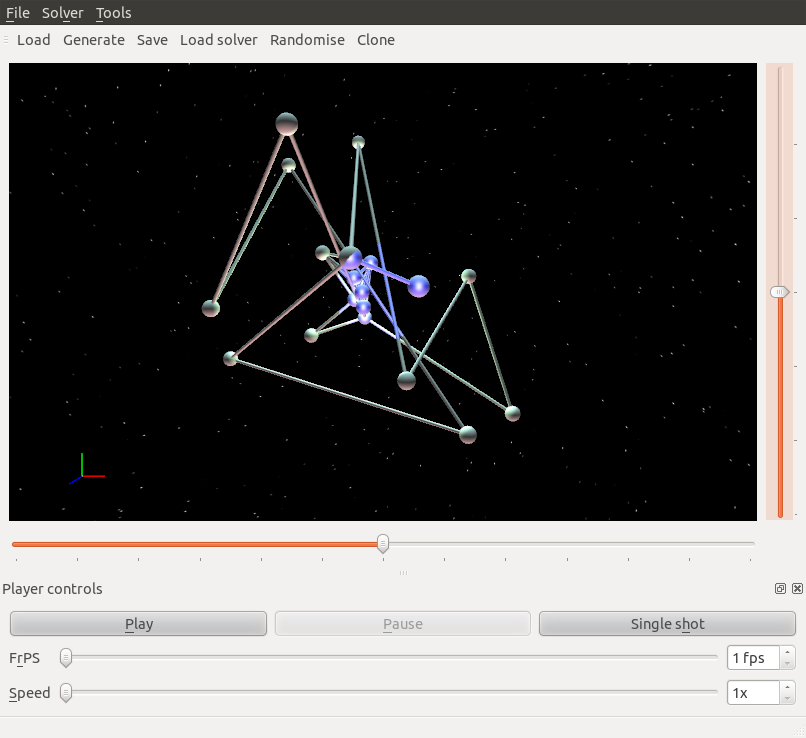
\includegraphics[width=0.8\textwidth]{screenshots/loaded.png}
	\end{center}
	\caption{Okno programu z~załadowanym grafem}
	\label{fig:scr:loaded}
\end{figure}

Do przemieszczania się w~tej przestrzeni służy urządzenie wskazujące.
Kliknięcie na panelu lewym przyciskiem i~przesuwanie wskaźnika w~pionie
przemieszcza kamerę w~pionie. Kliknięcie prawym przyciskiem i~przesuwanie
wskaźnika w~pionie przemieszcza kamerę w~przód i~w~tył
(przybliżenie, oddalenie). Kliknięcie lewym lub prawym przyciskiem
i~przesuwanie wskaźnika w~poziomie przemieszcza kamerę w~poziomie.

W~celu dokładnego ustawienia kamery można podczas przesuwania trzymać
wciśnięty klawisz Shift, co spowoduje spowolnienie ruchu kamery.
Analogicznie, aby przyspieszyć ruch kamery można przytrzymać wciśnięty
klawisz Ctrl.

Znajdujące się po prawej stronie oraz poniżej panelu suwaki umożliwiają
obroty kamery, odpowiednio w~osi poziomej i~pionowej.

\subsubsection{Ustawienia programu}

Program posiada kilka ustawień, które mogą być zmieniane przez użytkownika,
które wpływają na proces wyświetlania i~przemieszczania kamery w~ramach
sceny. Modyfikować można je po otwarciu okna ustawień programu (opcja
w~menu górnym).

Okno ustawień (rysunek \ref{fig:scr:settings}) programu to jedno z~wielu
wykonanych w~analogiczny sposób okien konfiguracyjnych. Zmiana ustawień
następuje w~momencie interakcji z~kontrolką (widgetem) umożliwiającą edycję
wartości, bez potrzeby potwierdzania. W~ten sposób, można mieć otwarte okno
ustawień dowolnego elementu (np. całego programu) i~zmieniać parametry
w~trakcie trwającej symulacji, obserwując na bieżąco efekty tych zmian.

\begin{figure}[tpb]
	\begin{center}
		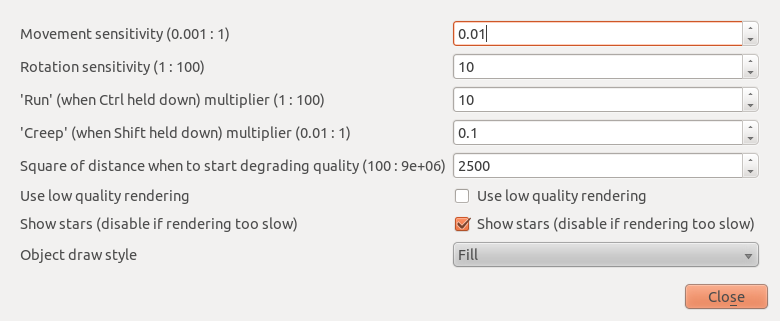
\includegraphics[width=0.8\textwidth]{screenshots/settings.png}
	\end{center}
	\caption{Okno ustawień programu}
	\label{fig:scr:settings}
\end{figure}

Ustawienia programu są współdzielone pomiędzy wszystkimi oknami programu.

\subsubsection{Uruchamianie symulacji}

Aby uruchomić symulację, należy wybrać jeden z~algorytmów wizualizacji
grafu, tzw. solver. Wciśnięcie przycisku ,,Load solver'' (lub wybranie
odpowiedniej opcji z~menu) spowoduje otwarcie modalnego okna dialogowego,
za pomocą którego z~listy należy wybrać jeden z~algorytmów.

Dostępne są 2 algorytmy: ForceSolver, działający w~oparciu o~fizyczny model
wizualizacji grafu, oraz EvolutionarySolver, działający w~oparciu o~model
ewolucyjny.

Po załadowaniu, każdy z~solverów wyświetla, w~dolnej części okna, dokowalną
kontrolkę umożliwiającą interakcje z~symulacją, w~szczególności
uruchamianie, zatrzymywanie, ustawienie szybkości odświeżania ekranu
(w~klatkach na sekundę) oraz szybkości symulacji (w~iteracjach na sekundę).
Kontrolkę tę można zamykać i~otwierać w~razie potrzeby, m.in. za pomocą
opcji menu ,,Solver $\rightarrow$ Solver Player''.

W~każdej chwili można (bezpowrotnie) zmienić algorytm. Spowoduje to
zatrzymanie symulacji i~załadowanie nowego wybranego solvera. Nowy algorytm
będzie traktował zastany stan tak, jakby był to graf wczytany z~pliku lub
wygenerowany, nie będzie ,,pamiętał'' operacji wykonanych poprzednim
solverem, nawet, jeśli był tego samego rodzaju. W~tym sensie jest to
operacja bezpowrotna.

\subsubsection{Ustawienia algorytmu}

Każdy z~algorytmów ma własny zestaw ustawień, obsługiwany w~analogiczny
sposób jak ustawienia programu. Okno ustawień można otworzyć za pomocą
opcji menu ,,Solver $\rightarrow$ Solver Settings''.

Ustawienia algorytmu nie są współdzielone. Każdy nowo załadowany solver
posiada domyślne ustawienia, nawet, jeśli solver tego samego rodzaju był
już wcześniej załadowany.

\subsubsection{Koniec symulacji}

Algorytm korzystający z~modelu fizycznego przerwie symulację w~momencie
osiągnięcia minimum energii układu, czyli w~sytuacji, w~której wszystkie
siły się równoważą. Jest to rozwiązanie zadania wizualizacji.

Algorytm ewolucyjny nie przerwie symulacji, ze względu na losowy i~ciągły
charakter obliczeń, wobec tego należy ręcznie przerwać symulację
w~sytuacji, kiedy prezentowany wynik będzie satysfakcjonujący.

\begin{figure}[tpb]
	\begin{center}
		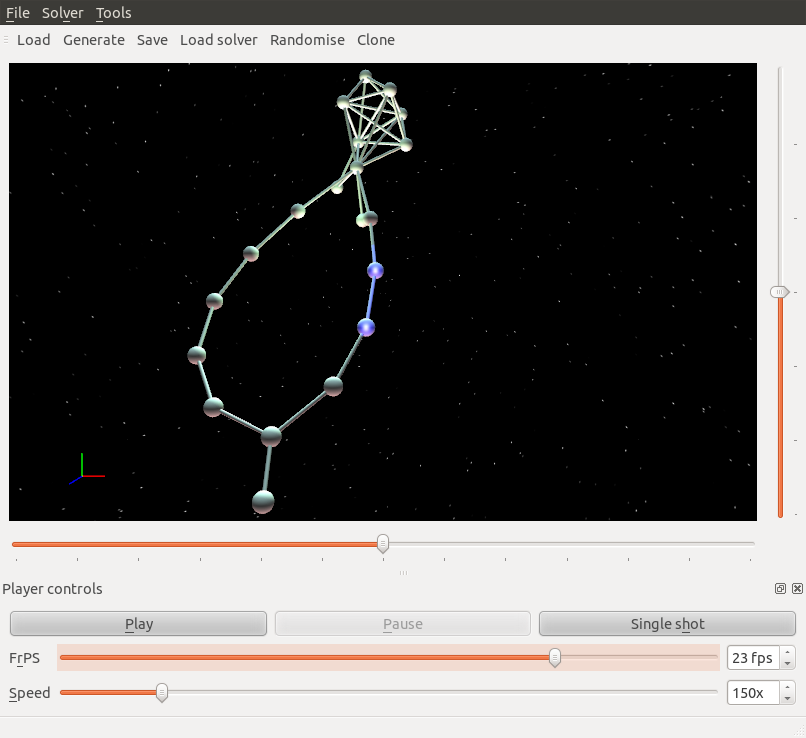
\includegraphics[width=0.8\textwidth]{screenshots/solved.png}
	\end{center}
	\caption{Okno programu po zakończeniu zadania wizualizacji grafu}
	\label{fig:scr:solved}
\end{figure}

\subsection{Parametry konfiguracyjne}

Listę parametrów konfiguracyjnych zamieszczamy na końcu sprawozdania.

\section{Badanie optymalnych parametrów algorytmu ewolucyjnego}

W~poszukiwaniu optymalnych naszym zdaniem parametrów algorytmu ewolucyjnego
posłużyliśmy się doświadczeniem, intuicją, a~następnie metodą inżynierską
próbowaliśmy poprawić te wartości. Uzyskane wartości parametrów ustawiliśmy
w~programie jako wartości domyślne. Następnie przeprowadziliśmy badania
pojedynczych parametrów w~celu znalezienia zależności i~możliwych kierunków
poprawy.

Na potrzeby badań wygenerowaliśmy jeden graf, który był następnie
wizualizowany przy różnych parametrach algorytmu ewolucyjnego.
Każda symulacja była uruchomiona od tego samego stanu początkowego i~trwała
milion iteracji. Funkcja celu dla wszystkich badań była również taka sama.

Przeprowadziliśmy następujące symulacje:

\begin{itemize}
	\item parametry domyślne: liczebność populacji 20, selekcja trywialna,
		krzyżowanie arytmetyczne uśredniające ($p=0,1$), mutacja ($p=0,7$,
		$\delta=0.1$), sukcesja elitarna
	\item prawdopodobieństwa krzyżowana: $p=0,7$
	\item algorytm krzyżowania: arytmetyczne losowe
	\item algorytm krzyżowania: wymianę genów
	\item parametry mutacji: $p=0.7$, $\delta=1$
	\item parametry mutacji: $p=0.3$, $\delta=1$
	\item liczebność populacji: 100
	\item liczebność populacji: 500
	\item selekcja: proporcjonalna
	\item selekcja: proporcjonalna i~liczebność populacji: 100
	\item selekcja: proporcjonalna i~liczebność populacji: 500
	\item selekcja: losowa o~rozkładzie jednostajnym
	\item selekcja: turniejowa $k=2$
	\item sukcesja: prosta
	\item sukcesja: unia elit $r=0.5$
\end{itemize}

Wyniki tych symulacji zostały przedstawione na wykresach, na końcu
sprawozdania.

\section{Podsumowanie i~wnioski}

W~naszym projekcie zawarliśmy dwa podejścia do zagadnienia wizualizacji 3D
grafu -- model fizyczny i~ewolucyjny. Zanim jednak przejdziemy do
porównania, chcemy przybliżyć rozważane zagadnienie.

Wizualizacja 3D grafu to zagadnienie dość skomplikowane, głównie ze względu
na określenie mierzalnych kryteriów jakości wizualizacji, konkretnej
funkcji oceny. W~modelu ewolucyjnym funkcja ta jest określana wprost i~na
jej podstawie następuje poszukiwanie rozwiązań, natomiast w~modelu
fizycznym funkcja ta nie jest dana wprost, lecz można ją intuicyjnie
utożsamić z~energią potencjalną oddziaływań całego układu.

Eksperymenty z~różnymi postaciami funkcji oceny w~modelu ewolucyjnym
doprowadziły nas do oczywistego wniosku -- funkcja oceny musi mieć co
najmniej jedno ,,wyraźne'' minimum, wokół którego funkcja wyraźnie rośnie,
w~przeciwnym wypadku znalezienie minimum w~jego sąsiedztwie jest bardzo
trudne. Jest to zgodne z~intuicją, albowiem siłą algorytmu ewolucyjnego
jest eksploracja i~wychodzenie poza zbiory przyciągania optimów lokalnych,
a~nie ,,dociąganie'' rozwiązania do samego optimum.

Bazując na tym wniosku, ograniczyliśmy znacznie liczbę możliwych postaci
funkcji celu do takich funkcji, które są złożeniem funkcji odpychania
Kulombowskiego oraz przyciągania grawitacyjnego bądź sprężystego.

Gdy w~świecie rzeczywistym rozważymy dwa jednoimiennie naładowane ciała
o~określonych masach znajdujące się w~położeniu równowagi pomiędzy siłami
przyciągania i~odpychania, jest oczywiste, że znajdują się w~pewnej
określonej odległości od siebie. Odległość ta wynika z~wartości ładunków,
mas, a~także stałych fizycznych. W~świecie symulacji ładunki są identyczne,
masy identyczne a~zamiast stałych fizycznych charakterystycznych dla
pojedynczych oddziaływań pojawia się pojęcie ,,pożądanej odległości''
pomiędzy parą wierzchołków w~równowadze. Owa ,,pożądana odległość'' to nie
jest jakieś uproszczenie na potrzeby symulacji, tylko konsekwencja
przyjętego modelu, w~którym wartość ta może być ustalona wprost (albowiem
kontrolujemy wszystkie stałe fizyczne symulacji).

Analogiczna wielkość w~modelu ewolucyjnym ukryta jest w~funkcji oceny.
Przyjmując funkcję oceny:
\begin{displaymath}
	f(x) = |a - x|^b + \frac{c}{x - d}
\end{displaymath}

Gdzie $x$ to odległość między rozpatrywaną parą wierzchołków, parametr $a$
ma kluczowy wpływ na faktyczną wartość ukrytej ,,pożądanej odległości''.

\subsection{Porównanie wyników}

Zdecydowanie lepsze rezultaty i~w~znacznie krótszym czasie osiągane są przy
zastosowaniu modelu fizycznego. Wynika to stąd, że niejawna funkcja celu
(minimum energii potencjalnej) jest funkcją wypukłą, zaś sama metoda
fizyczna jest analogiem metody gradientowej. W~każdej iteracji, na podstawie
działających sił wyliczany jest wektor zmian w~kierunku gradientu funkcji
celu. Od zwykłej metody gradientowej model fizyczny różni się tym, że
wprowadzone są pewne bezwładności, które występują w~świecie fizycznym, na
podstawie którego model jest wzorowany. W~związku z~tym podobieństwem do
metod gradientowych, odnalezienie minimum jest bardzo szybkie, a~ponieważ
niejawna funkcja celu ma bardzo niskie prawdopodobieństwo posiadania
minimów lokalnych, rozwiązanie generowane przy pomocy tego modelu zwykle
jest optymalne.

Model ewolucyjny dla prostych, zaprojektowanych jako przewidywalne
przykładów zachowuje się dobrze, pod warunkiem przyjęcie odpowiedniej
funkcji celu. Model znajduje rozwiązanie bliskie optymalnemu w~stosunkowo
krótkim czasie. Niestety model ten nie radzi sobie ze skomplikowanymi
grafami generowanymi losowo.

\subsubsection{Uwagi do strategii ewolucyjnej}

Przyjęta przez nas funkcja celu jest często funkcją unimodalną (dla drzew
i~nieskomplikowanych grafów), w~związku z~czym eksploracja przy pomocy
krzyżowania nie daje korzyści większych, niż lokalne, na dobrą sprawę
losowe, przeszukiwanie przestrzeni przy zastosowaniu mutacji o~małym
zasięgu. Z~rysunku \ref{fig:plot:cross} widać wyraźnie, że korzystne jest
stosowanie jedynie krzyżowania arytmetycznego o~stosunkowo małym
prawdopodobieństwie. Widać również, że krzyżowanie arytmetyczne
uśredniające okazało się bardziej korzystne niż krzyżowanie arytmetyczne
losowe.

Warto zauważyć (na rysunku \ref{fig:plot:proportional}), że selekcja
proporcjonalna dała pewną poprawę przy stosunkowo małej liczebności
populacji. Jest to spowodowane tym, że funkcja celu słabo różnicuje podobne
osobniki, co powoduje, że mechanizm selekcji proporcjonalnej bardzo
nieznacznie promuje osobniki lepiej dostosowane. Efekty takiej selekcji
będą bardzo zbliżone do efektów selekcji z~rozkładem równomiernym.

Na rysunku \ref{fig:plot:selection-2} widać wyraźnie, że dla małej
liczebności populacji selekcja proporcjonalna daje efekty znacznie lepsze
od selekcji trywialnej.

\subsection{Generowanie grafów}

Warto wspomnieć jeszcze słowem o~generowaniu grafów. Jak się okazuje,
generowanie grafów nie jest zadaniem trywialnym. Istnieje wiele metod
generowania grafów, jednakże uzyskiwanie grafów o~konkretnych pożądanych
właściwościach jest już trudne. Przejrzeliśmy literaturę, głównie artykuły
naukowe, na temat różnych podejść do generowania grafów i~wybraliśmy te,
które naszym zdaniem są jednocześnie dość proste i~dają pożądane rezultaty.
Jak się okazuje, spójność grafu jest dość trudnym warunkiem do spełnienia
przez generator, dlatego posłużyliśmy się pomocniczą strukturą zbiorów
rozłącznych do losowego uspójnienia grafu (połączenia reprezentantów
składowych w~ścieżkę).

\section{Literatura}

Poniżej zamieszczamy niewyczerpującą i~nieostateczną listę pozycji
literaturowych, które zostały przez nas zastosowane.

\begin{itemize}
	\item Grafy i~Sieci (GIS) -- notatki z~wykładów
	\item \url{http://en.wikipedia.org/wiki/Geometric\_graph\_theory}
	\item \url{http://en.wikipedia.org/wiki/Erd\%C5\%91s\%E2\%80\%93R\%C3\%A9nyi\_model}
	\item Filip Piękniewski, Wydział Matematyki i~Informatyki, UMK,
		Prezentacja na Seminarium Doktoranckie dostępna na
		\url{http://www.mat.uni.torun.pl/~philip/sem-2008-2.pdf}
	\item
		\url{http://en.wikipedia.org/wiki/Force-based\_algorithms\_\%28graph\_drawing\%29}

\end{itemize}


\section*{Parametry konfiguracyjne programu i~algorytmów}

Poniżej zamieszczamy spis wszystkich parametrów konfiguracyjnych programu
i~jego składników.

\begin{table}[h!]
	\centering
	\begin{tabular}{p{0.38\textwidth}p{0.58\textwidth}}
		\hline
Movement sensitivity & Czułość przemieszczania kamery \\
Rotation sensitivity & Czułość obrotu kamery \\
'Run' multiplier & Współczynnik przyspieszenia ruchu kamery (podczas wciskania klawisza Ctrl) \\
'Creep' multiplier & Współczynnik spowolnienia ruchu kamery (podczas wciskania klawisza Shift) \\
Square of distance when to start degrading quality & Kwadrat odległości zasięgu kamery \\
Show names above objects & Wyświetlanie nazw obiektów \\
Display textures & Wyświetlanie tekstur \\
Use low quality rendering & Włączenie trybu wyświetlania w niskiej jakości \\
Show stars & Wyświetlanie gwiazd w tle sceny \\
Object draw style & Sposób rysowania obiektów \\
		\hline
	\end{tabular}
	\caption{Parametry programu}
	\label{tab:params-program}
\end{table}

\begin{table}[h!]
	\centering
	\begin{tabular}{p{0.38\textwidth}p{0.58\textwidth}}
		\hline
Number of nodes & Liczba wierzchołków \\
Proximity radius & Promień sąsiedztwa (0.0-1.0) \\
Scale & Współczynnik skali przestrzeni \\
		\hline
	\end{tabular}
	\caption{Parametry generatora sieci Euklidesowych}
	\label{tab:params-gen-ecn}
\end{table}

\begin{table}[h!]
	\centering
	\begin{tabular}{p{0.38\textwidth}p{0.58\textwidth}}
		\hline
Number of nodes & Liczba wierzchołków \\
		\hline
	\end{tabular}
	\caption{Parametry generatora Euklidesowych minimalnych drzew
	rozpinających}
	\label{tab:params-gen-tree}
\end{table}

\begin{table}[h!]
	\centering
	\begin{tabular}{p{0.38\textwidth}p{0.58\textwidth}}
		\hline
Number of nodes & Liczba wierzchołków \\
Edge probability & Prawdopodobieństwo krawędzi \\
Radius & Współczynnik skali przestrzeni \\
		\hline
	\end{tabular}
	\caption{Parametry generatora Erdos-Renyi}
	\label{tab:params-gen-er}
\end{table}

\begin{table}[h!]
	\centering
	\begin{tabular}{p{0.38\textwidth}p{0.58\textwidth}}
		\hline
Population size & Liczebność populacji \\
Selection type & Algorytm selekcji \\
Selection: k-param & Parametr $k$ algorytmu selekcji \\
Crossover probability & Prawdopodobieństwo krzyżowania \\
Crossover type & Algorytm krzyżowania \\
Mutation probability & Prawdopodobieństwo mutacji \\
Mutation standard deviation & Odchylenie standardowe mutacji \\
Succession type & Algorytm sukcesji \\
Evaluation Func for adjacent & Składnik funkcji oceny dla wierzchołków sąsiednich \\
EvF-adjacent, param a & Parametr $a$ f. oceny dla wierzchołków sąsiednich \\
EvF-adjacent, param a & Parametr $b$ f. oceny dla wierzchołków sąsiednich \\
Evaluation Func for non-adjacent & Składnik funkcji oceny dla wierzchołków niesąsiednich \\
EvF-non-adjacent, param a & Parametr $a$ f. oceny dla wierzchołków niesąsiednich \\
EvF-non-adjacent, param a & Parametr $b$ f. oceny dla wierzchołków niesąsiednich \\
Evaluation Func for all pairs & Składnik funkcji oceny dla wszystkich par wierzchołków \\
EvF-all, param a & Parametr $a$ f. oceny dla wszystkich par wierzchołków \\
EvF-all, param a & Parametr $b$ f. oceny dla wszystkich par wierzchołków \\
		\hline
	\end{tabular}
	\caption{Parametry solvera ewolucyjnego}
	\label{tab:params-solver-evo}
\end{table}

\begin{table}[h!]
	\centering
	\begin{tabular}{p{0.38\textwidth}p{0.58\textwidth}}
		\hline
Repulsion force & Współczynnik siły odpychania \\
Attraction force & Współczynnik siły przyciągania \\
Repulsion when nodes are very near & Współczynnik siły odpychania dla bliskich wierzchołków \\
Force towards the center & Współczynnik siły przyciągania względem centrum sceny \\
Desired edge length & Pożądana odległość między sąsiednimi wierzchołkami \\
Damping & Współczynnik tłumienia \\
Move limit & Ograniczenie maksymalnego przemieszczenia w jednej iteracji \\
Velocity limit & Ograniczenie prędkości \\
dt per iteration & Wielkość kwantu czasu w iteracji \\
Attraction proportional to degree & Przyciąganie proporcjonalne do stopnia wierzchołka \\
		\hline
	\end{tabular}
	\caption{Parametry solver fizycznego}
	\label{tab:params-solver-force}
\end{table}

\clearpage


\section*{Wykresy do badań parametrów algorytmu ewolucyjnego}

Poniżej zamieszczamy wykresy do badań parametrów algorytmu ewolucyjnego.

\begin{figure}[hp]
	\begin{center}
		\includegraphics{out/cross}
	\end{center}
	\caption{Różne wyniki krzyżowania}
	\label{fig:plot:cross}
\end{figure}

\begin{figure}[hp]
	\begin{center}
		\includegraphics{out/proportional}
	\end{center}
	\caption{Selekcja proporcjonalna dla różnych liczebności populacji}
	\label{fig:plot:proportional}
\end{figure}

\begin{figure}[hp]
	\begin{center}
		\includegraphics{out/population}
	\end{center}
	\caption{Różne liczebności populacji}
	\label{fig:plot:population}
\end{figure}

\begin{figure}[hp]
	\begin{center}
		\includegraphics{out/selection}
	\end{center}
	\caption{Różne algorytmy selekcji}
	\label{fig:plot:selection}
\end{figure}

\begin{figure}[hp]
	\begin{center}
		\includegraphics{out/selection-2}
	\end{center}
	\caption{Dokładniejsze porównani selekcji trywialnej i~proporcjonalnej
	(liczebność populacji $20$ osobników).}
	\label{fig:plot:selection-2}
\end{figure}

\begin{figure}[hp]
	\begin{center}
		\includegraphics{out/succession}
	\end{center}
	\caption{Porównanie sukcesji elitarnej z~sukcesją typu ,,unia elit''
	(po połowie najlepiej dostoswanych osobników z~populacji bazowej
	i~pokolenia potomnego)}
	\label{fig:plot:succession}
\end{figure}

\begin{figure}[hp]
	\begin{center}
		\includegraphics{out/straight}
	\end{center}
	\caption{Sukcesja prosta -- wyraźnie nieefektywna}
	\label{fig:plot:straight}
\end{figure}

\begin{figure}[hp]
	\begin{center}
		\includegraphics{out/mutation}
	\end{center}
	\caption{Różne parametry mutacji}
	\label{fig:plot:mutation}
\end{figure}

\end{document}

